% !TeX spellcheck = en_GB
\ifcsname SlidesDistr\endcsname%
\documentclass[handout,aspectratio=169]{beamer}
\else%
\documentclass[aspectratio=169]{beamer}
\fi%
\usepackage{fontspec}
\usepackage[T1]{fontenc}
\usepackage{amsmath}
\usepackage{amsfonts}
\usepackage{amssymb}
\usepackage{graphicx}
\usepackage{csquotes}
\usepackage{booktabs}
\usepackage{multicol}
\usepackage{enumerate}
\usepackage{microtype}
\usepackage[labelfont=bf,font={small}]{caption}
\usepackage{hyperref}
\usepackage{booktabs}
\usepackage{subcaption}
\usepackage{fancyhdr}
\usepackage{pdfpages}
\usepackage{siunitx}
\usepackage{tikz}
\usepackage{mdframed}

\defaultfontfeatures{Mapping=tex-text}
\newfontfamily\symbolfont{Symbola}
\newfontfamily\quotefont{GentiumPlus}

\usepackage[sorting=none]{biblatex}
\addbibresource{../bibliography.bib}

\author{Chris Eliasmith}


\renewcommand{\vec}[1]{{\mathbf{#1}}}
\newcommand{\mat}[1]{{\mathbf{#1}}}
\newcommand{\T}{\ensuremath{\mathsf{T}}}
\renewcommand{\epsilon}{\varepsilon}
\renewcommand{\phi}{\varphi}

% Tango color palette
\definecolor{butter1}{HTML}{FCE94F}
\definecolor{butter2}{HTML}{EDD400}
\definecolor{butter3}{HTML}{C4A000}
\definecolor{orange1}{HTML}{FCAF3E}
\definecolor{orange2}{HTML}{F57900}
\definecolor{orange3}{HTML}{CE5C00}
\definecolor{chocolate1}{HTML}{E9B96E}
\definecolor{chocolate2}{HTML}{C17D11}
\definecolor{chocolate3}{HTML}{8F5902}
\definecolor{chameleon1}{HTML}{8AE234}
\definecolor{chameleon2}{HTML}{73D216}
\definecolor{chameleon3}{HTML}{4E9A06}
\definecolor{skyblue1}{HTML}{729FCF}
\definecolor{skyblue2}{HTML}{3465A4}
\definecolor{skyblue3}{HTML}{204A87}
\definecolor{plum1}{HTML}{AD7FA8}
\definecolor{plum2}{HTML}{75507B}
\definecolor{plum3}{HTML}{5C3566}
\definecolor{scarletred1}{HTML}{EF2929}
\definecolor{scarletred2}{HTML}{CC0000}
\definecolor{scarletred3}{HTML}{A40000}
\definecolor{aluminium1}{HTML}{EEEEEC}
\definecolor{aluminium2}{HTML}{D3D7CF}
\definecolor{aluminium3}{HTML}{BABDB6}
\definecolor{aluminium4}{HTML}{888A85}
\definecolor{aluminium5}{HTML}{555753}
\definecolor{aluminium6}{HTML}{2E3436}

\definecolor{violet}{HTML}{AA305C}
\definecolor{uwyellow}{HTML}{FDD433}
\definecolor{background}{HTML}{F9F9F6}
\definecolor{text}{HTML}{000000}

\definecolor{uweng1}{HTML}{D1B2EE}
\definecolor{uweng2}{HTML}{BF33DE}
\definecolor{uweng3}{HTML}{8001B3}
\definecolor{uweng4}{HTML}{56048A}

\setbeamercolor{title}{fg=violet}
\setbeamercolor{frametitle}{fg=black}
\setbeamercolor{structure}{fg=aluminium5}
\setbeamercolor{normal text}{fg=text}

\setbeamertemplate{navigation symbols}{}
\setbeamertemplate{footline}[frame number]

\hypersetup{%
	colorlinks=false,% hyperlinks will be black
	urlbordercolor=aluminium4,% hyperlink borders will be red
	pdfborderstyle={/S/U/W 0.5}% border style will be underline of width 1pt
}

\makeatletter
\newcommand{\superimpose}[2]{%
	{\ooalign{{#1}\hidewidth\cr{#2}\hidewidth\cr}}}
\makeatother
\newcommand{\SolidCircle}[2]{\superimpose{\color{#1}\symbolfont ⬤}{\textbf{\color{white}#2}}\hspace{1em}}
\newcommand{\OPlus}{\SolidCircle{chameleon3}{\kern0.75pt+}}
\newcommand{\OMeh}{\SolidCircle{uwyellow}{~}}
\newcommand{\OMinus}{\SolidCircle{scarletred3}{\kern2.25pt--}}

\newcommand{\hl}[1]{\colorbox{uwyellow}{{\color{black}\textbf{#1}}}}

\newcommand{\ImageSources}[1]{%
	\begin{columns}%
		\column{1.1\textwidth}%
		\raggedright%
		\tiny\color{aluminium4}%
		\setlength\lineskip{1em}%
		\textbf{Image Sources.}	{#1}%
	\end{columns}}

\newcommand{\ColorRect}[3]{{\color{#1}\rule{#2}{#3}}}
\setbeamertemplate{headline}{\ColorRect{black}{\textwidth}{4pt}\newline\ColorRect{uweng1}{0.25\textwidth}{4pt}\ColorRect{uweng2}{0.25\textwidth}{4pt}\ColorRect{uweng3}{0.25\textwidth}{4pt}\ColorRect{uweng4}{0.25\textwidth}{4pt}}

\newcommand{\MakeTitle}{%
	\vspace{0.5cm}%
	{\textbf{\inserttitle}}\\[0.5cm]%
	\insertauthor\\[0.5cm]%
	\insertdate\\%
	\begin{itemize}
		\item Slide design: Andreas Stöckel
		\item Content: Terry Stewart, Andreas Stöckel, Chris Eliasmith
	\end{itemize}
 	
\includegraphics[width=7cm]{../assets/uwlogo_eng.pdf}%
}

\newcommand{\handwritingframe}{%
	\begin{frame}
		\begin{columns}
			\column{\paperwidth}
			
\includegraphics{../assets/handwriting_lines.pdf}
		\end{columns}
	\end{frame}	
}

\newcommand{\imageframe}[1]{%
	\setbeamertemplate{navigation symbols}{}%
	\begin{frame}[plain,noframenumbering]%
		\begin{tikzpicture}[remember picture,overlay]%
		\node[at=(current page.center)] {%
			\includegraphics[width=\paperwidth]{#1}%
		};%
		\end{tikzpicture}%
	\end{frame}%
}

\newcommand{\videoframe}[3][mp4]{%
	\begin{frame}[plain,noframenumbering]%
		\hypersetup{%
			pdfborderstyle={/S/U/W 0}% border style will be underline of width 1pt
		}%
		\begin{tikzpicture}[remember picture,overlay]%
		\node[at=(current page.center)] {%
			\includegraphics[width=\paperwidth]{{video/#2_#3}.jpg}%
		};%
		\node[at=(current page.center)] {%
			\ifcsname SlidesDistr\endcsname%
				\href{https://youtu.be/#3}{
\includegraphics[width=2cm]{../assets/play_button.pdf}}%
			\else%
				\href{video/#2_#3.#1}{
\includegraphics[width=2cm]{../assets/play_button.pdf}}%
			\fi%
		};%
		\end{tikzpicture}%
	\end{frame}%
}

\newcommand{\includevideo}[4][mp4]{%
	\begingroup%
	\hypersetup{%
		pdfborderstyle={/S/U/W 0}% border style will be underline of width 1pt
	}%
	\begin{tikzpicture}%
	\node (A) {%
		\includegraphics[width=#4]{{video/#2_#3}.jpg}%
	};%
	\node[at=(A.center)] {%
		\ifcsname SlidesDistr\endcsname%
			\href{https://youtu.be/#3}{
\includegraphics[width=2cm]{../assets/play_button.pdf}}%
		\else%
			\href{video/#2_#3.#1}{
\includegraphics[width=2cm]{../assets/play_button.pdf}}%
		\fi%
	};%
	\end{tikzpicture}%
	\endgroup%
}

\newcommand{\backupbegin}{
	\newcounter{finalframe}
	\setcounter{finalframe}{\value{framenumber}}
	\setbeamertemplate{footline}{}
}

\newcommand{\backupend}{
	\setcounter{framenumber}{\value{finalframe}}
}


\date{October 16 \& 18, 2023}
\title{SYDE 556/750 \\ Simulating Neurobiological Systems \\ Lecture 6: Recurrent Dynamics}

\begin{document}
	
	\begin{frame}{}
		\vspace{0.5cm}
		\begin{columns}[c]
			\column{0.6\textwidth}
			\MakeTitle
			\column{0.4\textwidth}
			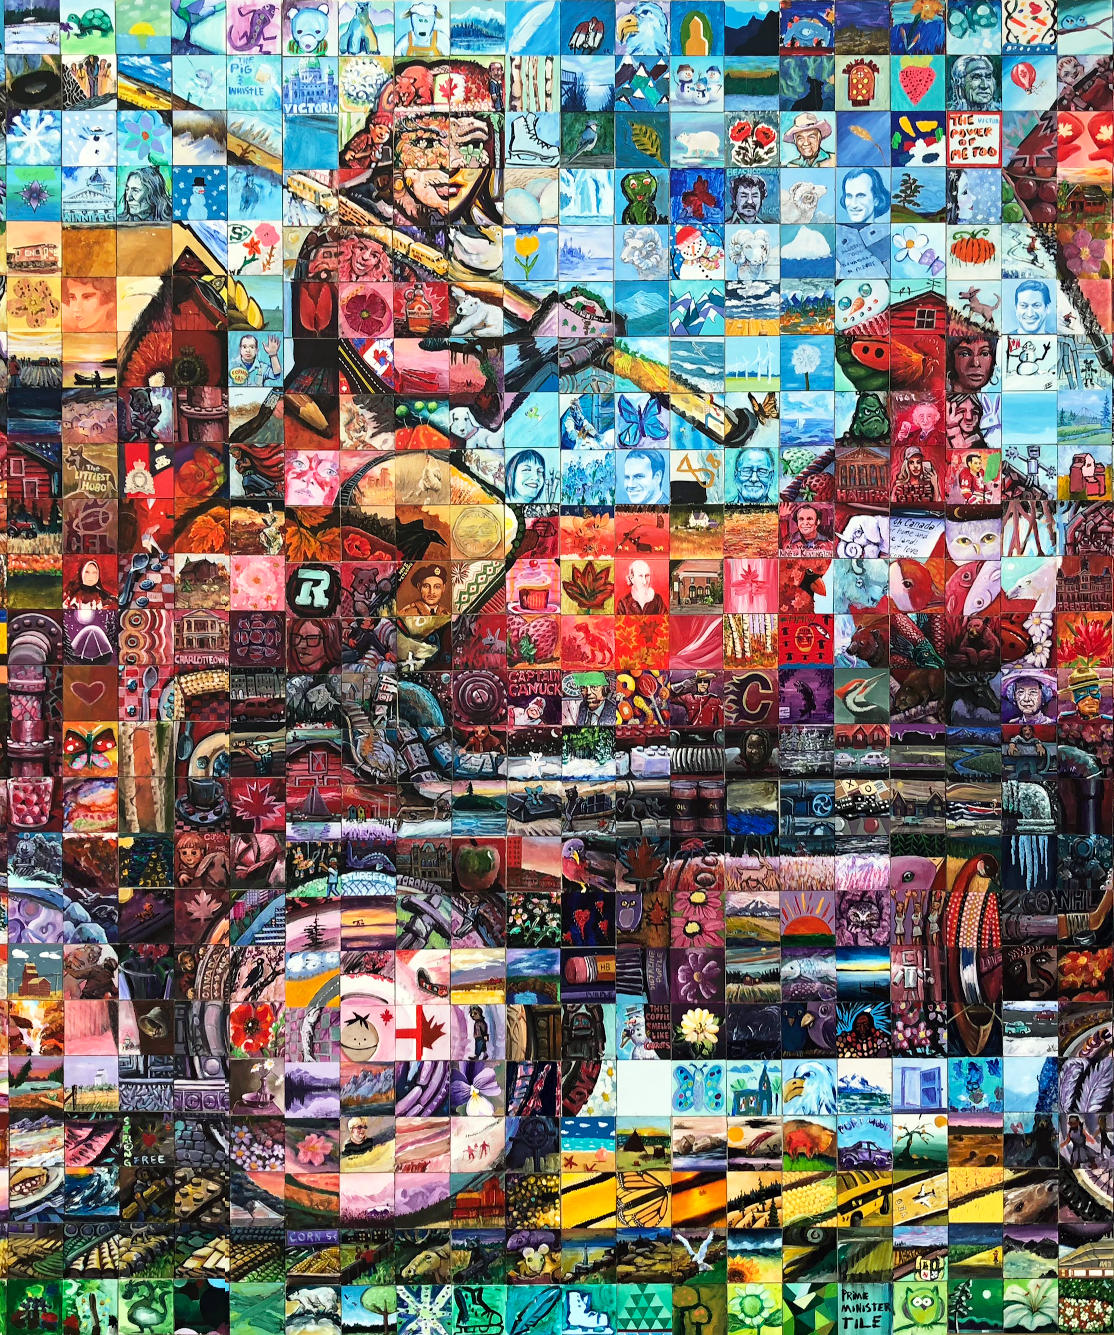
\includegraphics[width=\textwidth]{media/canada_150_mosaic_engine_small.jpg}
		\end{columns}
	\end{frame}

	\begin{frame}{Feed Forward vs. Recurrent Connections}
		\centering
		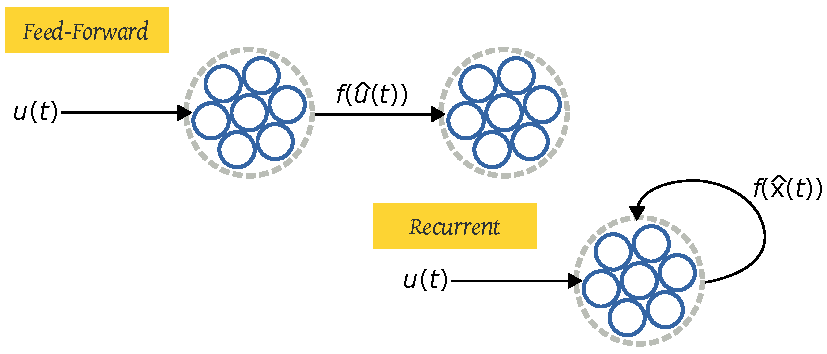
\includegraphics{media/feed_forward_recurrent.pdf}
	\end{frame}

	\begin{frame}{Recurrence Experiments (I)}
		\centering
		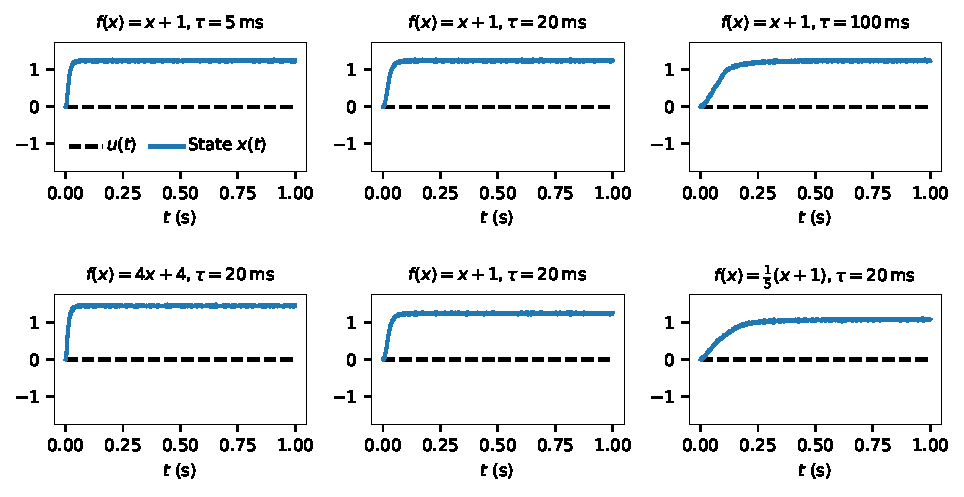
\includegraphics[width=\textwidth]{media/fxp1_example.pdf}
	\end{frame}

	\begin{frame}{Recurrence Experiments (II)}
		\centering
		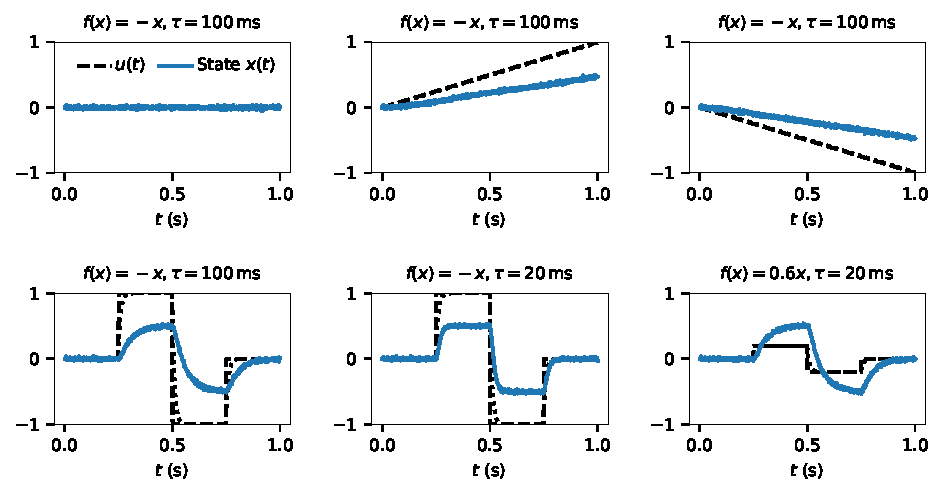
\includegraphics[width=\textwidth]{media/fmx_example.pdf}
	\end{frame}

	\begin{frame}{Recurrence Experiments (III)}
		\centering
		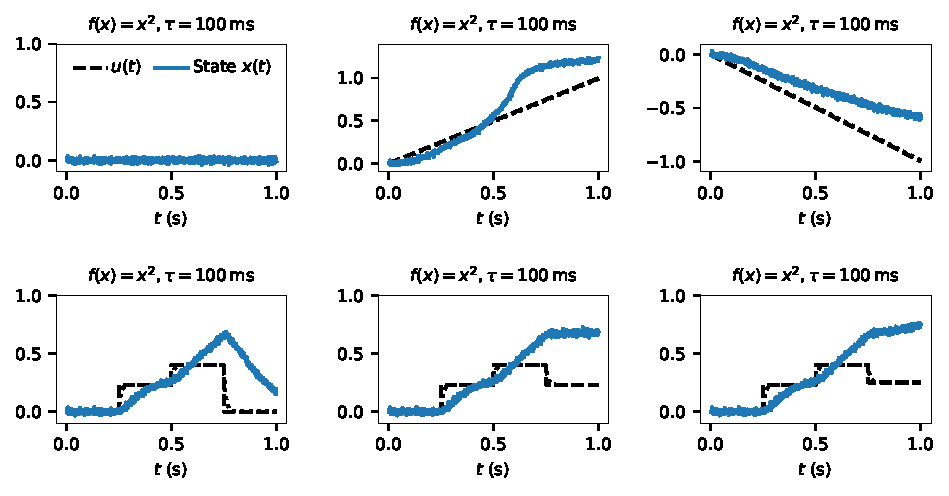
\includegraphics[width=\textwidth]{media/fxs_example.pdf}
	\end{frame}


	\begin{frame}{Making Sense of Dynamics}
		\centering
		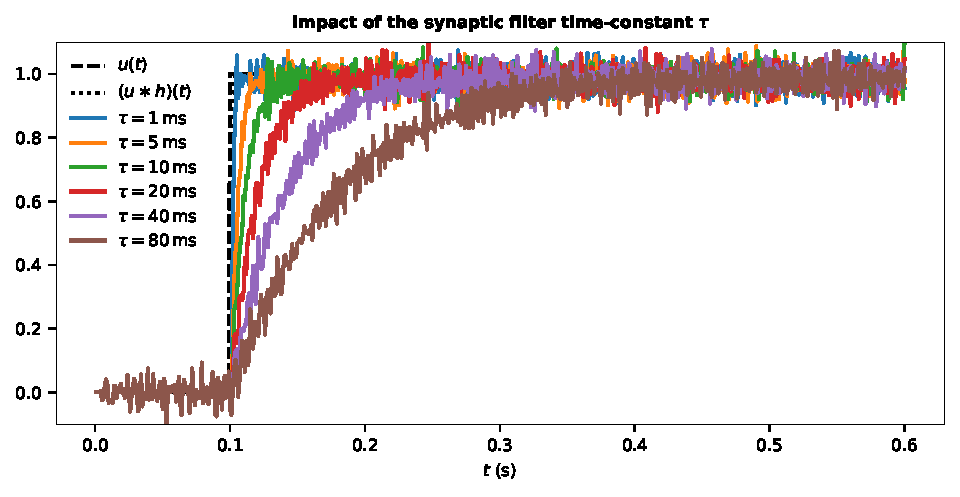
\includegraphics[width=\textwidth]{media/synaptic_filter.pdf} 		
	\end{frame}

	%\begin{frame}{Phase Portraits}
%		\centering
%		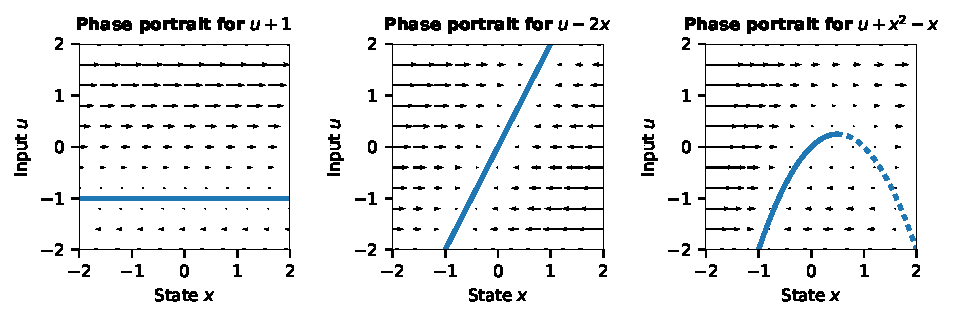
\includegraphics[width=\textwidth]{media/phase_portraits.pdf}
%	\end{frame}

	\begin{frame}{Behaviour of a Recurrent Connection}
	Feed-forward
			\begin{align*}
				x(t) = g(u(t)) * h(t)				
			\end{align*}		
	Recurrent
			\begin{align*}
	x(t) &= (g(u(t)) + f(x(t))) * h(t)	\\
	X(s) &= (G(s) + F(s))H(s) \\
	X(s) &= (G(s) + F(s)){1 \over {1+s\tau}} \\
	X(s) + s\tau X(s) &= G(s) + F(s) \\
	s\tau X(s) &= G(s) + F(s) - X(s) \\
	sX(s) &= {{F(s) - X(s)} \over \tau} + {G(s) \over \tau} \\
	{dx \over dt} &= {{f(x(t))-x(t)} \over \tau} + {{g(u(t))} \over \tau}
			\end{align*}		
	
	\end{frame}

	\begin{frame}{Behaviour of a Recurrent Connection}
	\begin{align*}
		{dx \over dt} &= {{f(x(t))-x(t)} \over \tau} + {{g(u(t))} \over \tau}
	\end{align*}		
	If we want this
	\begin{align*}
	{dx \over dt} &= a(x) + b(u)
	\end{align*}
	Then we set
	\begin{align*}
	f(x) &= \tau a(x) + x \\
	g(x) &= \tau b(u)
	\end{align*}
	And we get
	\begin{align*}
	{dx \over dt} &= {{(\tau a(x) + x) - x} \over \tau} + {{(\tau b(u))} \over \tau} \\
	{dx \over dt} &= {{a(x)}} + {{b(u)}}
	\end{align*}		
	
	
			
	
	
\end{frame}


	\begin{frame}{Implementing Dynamics using a Neural Ensemble}
		\centering
		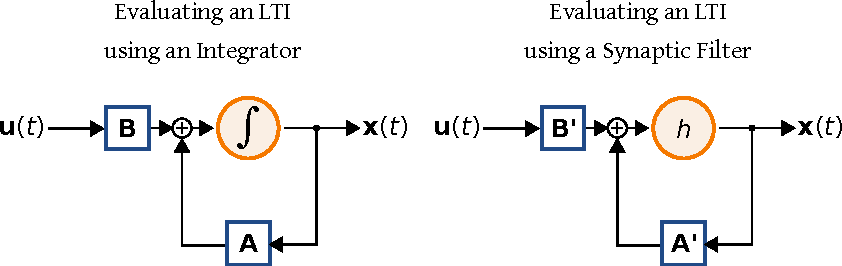
\includegraphics[width=\textwidth]{media/lti_integrator_vs_neural.pdf} 
	\end{frame}

	\begin{frame}{Implementing Dynamical Systems as a Neural Ensemble}
		\begin{columns}[t]
			\column{0.5\textwidth}
			\centering
			\hl{LTI System}
			\begin{align*}
				\phi(\vec u, \vec x) &= \mat A \vec x + \mat B \vec u \\
				\phi'(\vec u, \vec x) &= \mat A' \vec x + \mat B' \vec u \\
				\mat A' &= \tau \mat A + \mat I \\ \mat B' &= \tau \mat B \,.
			\end{align*}
			\column{0.5\textwidth}
			\centering
			\hl{Additive Time-Invariant System}
			\begin{align*}
				\phi(\vec u, \vec x) &= f(\vec x) + g(\vec u) \\
				\phi'(\vec u, \vec x) &= f'(\vec x) + g'(\vec u) \\
				f'(\vec x) &= \tau f(\vec x) + \vec x \\
				g'(\vec u) &= \tau g(\vec u)
			\end{align*}
		\end{columns}
		\vspace{1cm}
		\centering \hl{\enquote{General} Recipe}\\[0.25cm]
		Scale the original dynamics by $\tau$, add feedback $\vec x$
	\end{frame}

	\begin{frame}{NEF Principle 3: Dynamics}
	\begin{columns}[b]
		\column{0.5\textwidth}
		\centering
		\hl{Time-Invariant Dynamical System}\\
		\begin{align*}
			\frac{\mathrm{d}\vec x(t)}{\mathrm{d}t} &= f(\vec x(t), \vec u(t))
		\end{align*}
		\column{0.5\textwidth}
		\centering
		\hl{Linear Time-Invariant (LTI)}
		\hl{Dynamical System}
		\begin{align*}
			\frac{\mathrm{d}\vec x(t)}{\mathrm{d}t} &= \mat A \vec x + \mat B \vec u
		\end{align*}
	\end{columns}
	\vspace{0.75cm}
	\begin{mdframed}
		\textbf{NEF Principle 3 -- Dynamics}\\
		Neural dynamics are characterized by considering neural representations as control theoretic state variables. We can use control theory (and dynamical systems theory) to analyse and construct these systems.
	\end{mdframed}
\end{frame}

\begin{frame}{Low-pass Filter Example}
Desired behaviour
\begin{align*}
	{dx \over dt} = {{u - x} \over \tau_{desired}}	
\end{align*}
Feed-forward input
\begin{align*}
	g(u) &= \tau_{synapse} ({u \over \tau_{desired}}) \\
	g(u) &= {\tau_{synapse} \over \tau_{desired}} u	
\end{align*}
Recurrent
\begin{align*}
	f(x) &= \tau_{synapse} ({{-x} \over \tau_{desired}}) + x \\
	f(x) &= (1-{\tau_{synapse} \over \tau_{desired}})x			
\end{align*}	
\end{frame}	

	\begin{frame}{Integrator Example (I)}
		\centering
		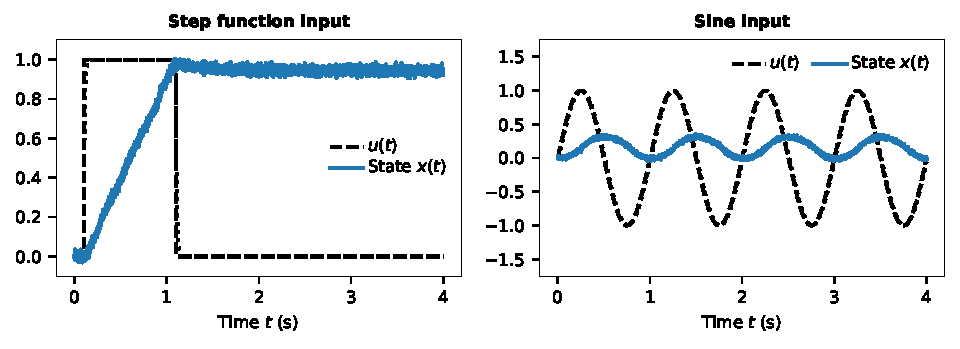
\includegraphics[width=\textwidth]{media/example_integrator.pdf}
	\end{frame}

	\begin{frame}{Integrator Example (II)}
		\centering
		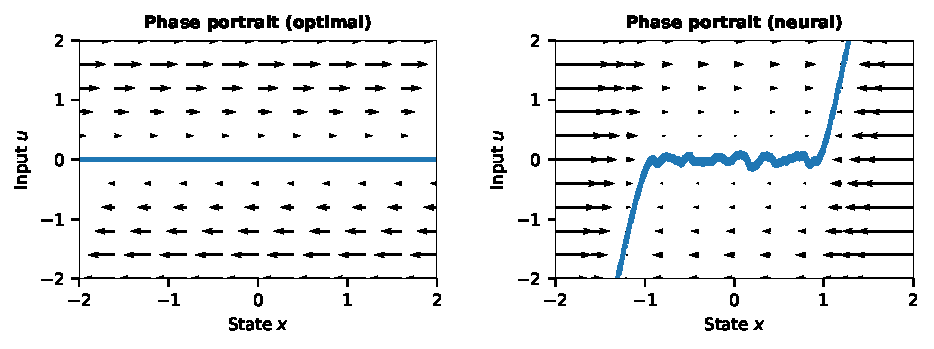
\includegraphics[width=\textwidth]{media/example_integrator_phases.pdf}
	\end{frame}

	\begin{frame}{Oscillator Example (I)}
		\centering
		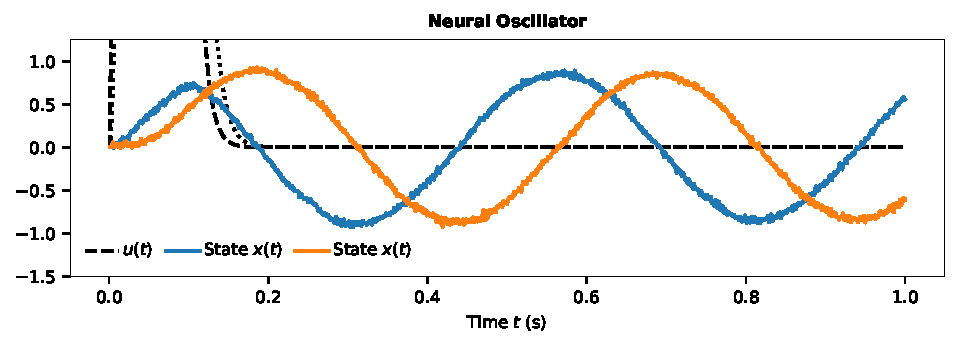
\includegraphics[width=\textwidth]{media/example_oscillator.pdf}
	\end{frame}

	\begin{frame}{Oscillator Example (II)}
		\centering
		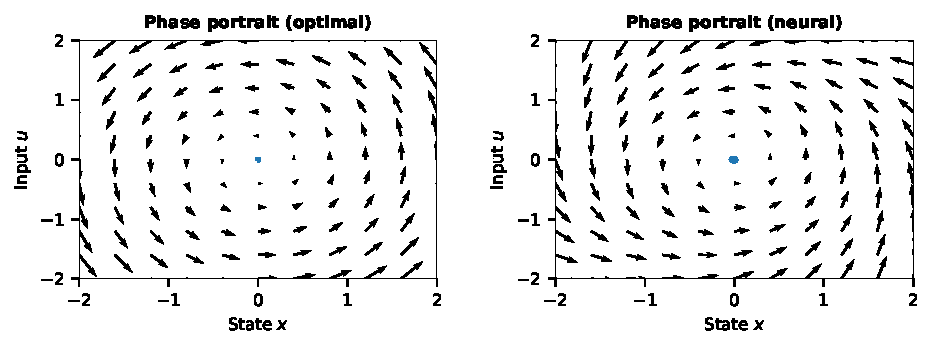
\includegraphics[width=\textwidth]{media/example_oscillator_phases.pdf}
	\end{frame}

	\begin{frame}{Lorentz Attractor}
		\centering
		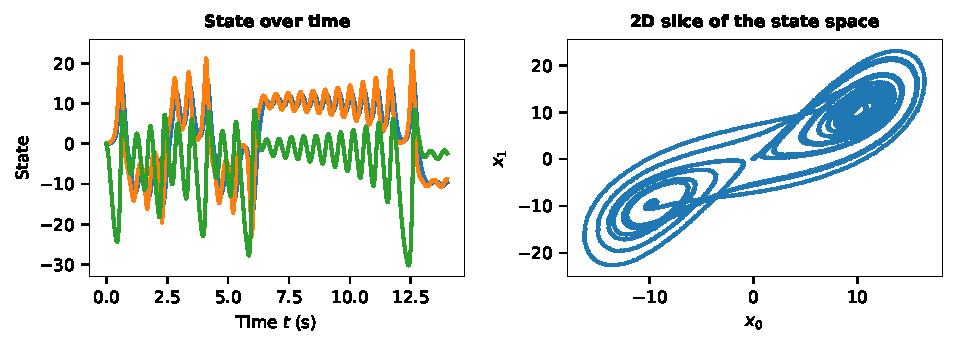
\includegraphics[width=\textwidth]{media/example_lorentz.pdf}
		\begin{align*}
			\frac{\mathrm{d}\vec x(t)}{\mathrm{d}t} &= \begin{pmatrix}
			10 x_2(t)-10x_1(t) \\
			-x_1(t) x_3(t)-x_2(t) \\
			x_1(t) x_2(t) - \frac{8}{3}(x_3(t)+28)-28
			\end{pmatrix}
		\end{align*}
	\end{frame}

	\begin{frame}{Heart Shape}
		\centering
		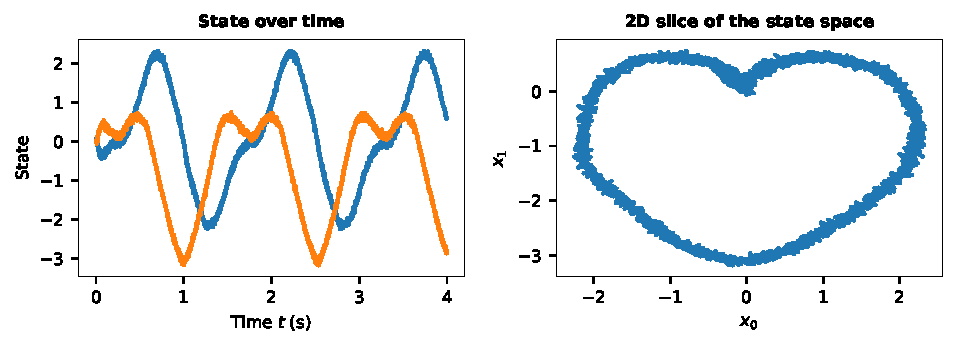
\includegraphics[width=\textwidth]{media/example_heart.pdf}
	\end{frame}

	\begin{frame}{Horizontal Eye Control}
		\centering
		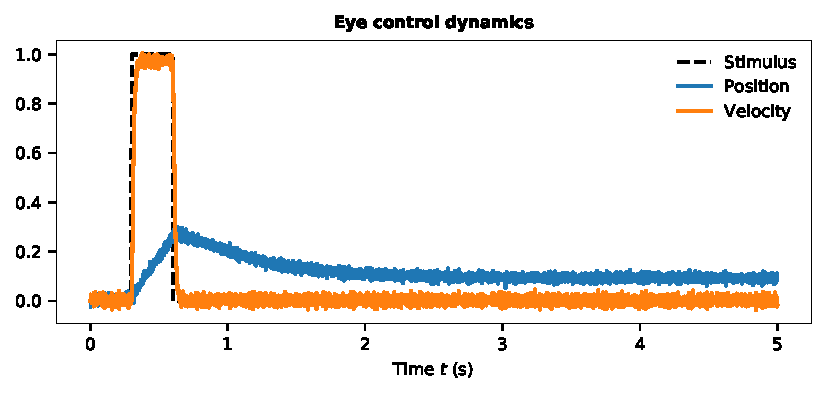
\includegraphics[width=\textwidth]{media/example_eye_control.pdf}
	\end{frame}

	\backupbegin

	\begin{frame}[noframenumbering]{Image sources}
		\small
		\textbf{Title slide}\\\enquote{The Canada 150 Mosaic Mural}\\Author: Mosaic Canada Murals.\\From \href{https://commons.wikimedia.org/wiki/File:Canada_150_Mosaic_Engine.jpg}{Wikimedia}.
	\end{frame}


	\backupend
	
\end{document}
